%=======================================================================
%  ICCIT 2026 -- CAMERA-READY version, 6 pages, IEEE conference format
%  From Spikes to Sentences: A Hybrid CTC Decoder with Confidence-Gated
%  Language Model Rescoring
%  Compile: pdflatex x3, with revision_results.tex in this folder.
%=======================================================================
\documentclass[conference,a4paper,10pt]{IEEEtran}
\IEEEoverridecommandlockouts

\usepackage{cite}
\usepackage{amsmath,amssymb}
\usepackage{graphicx}
\usepackage{booktabs}
\usepackage{multirow}
\usepackage{array}
\usepackage{balance}
\usepackage{xcolor}
\usepackage{tikz}
\usetikzlibrary{arrows.meta,positioning,calc,fit,backgrounds,shapes.geometric}
\usepackage{pgfplots}
\pgfplotsset{compat=1.17}
\usepackage{algorithm}
\usepackage{algpseudocode}
\usepackage{adjustbox}
\usepackage[hidelinks]{hyperref}

%-----------------------------------------------------------------------
%  Float placement discipline (see revision notes).
%-----------------------------------------------------------------------
\setcounter{topnumber}{3}
\setcounter{bottomnumber}{2}
\setcounter{totalnumber}{5}
\setcounter{dbltopnumber}{2}
\renewcommand{\topfraction}{0.92}
\renewcommand{\dbltopfraction}{0.92}
\renewcommand{\bottomfraction}{0.70}
\renewcommand{\textfraction}{0.06}
\renewcommand{\floatpagefraction}{0.72}
\renewcommand{\dblfloatpagefraction}{0.72}
\setlength{\textfloatsep}{8pt plus 2pt minus 2pt}
\setlength{\floatsep}{8pt plus 2pt minus 2pt}
\setlength{\intextsep}{8pt plus 2pt minus 2pt}
\setlength{\dbltextfloatsep}{8pt plus 2pt minus 2pt}
\setlength{\dblfloatsep}{8pt plus 2pt minus 2pt}
\setlength{\abovecaptionskip}{3pt}
\setlength{\belowcaptionskip}{0pt}

\definecolor{ioFill}{HTML}{ECEFF4}\definecolor{ioLine}{HTML}{4C566A}
\definecolor{acFill}{HTML}{E3EEF9}\definecolor{acLine}{HTML}{3B6EA5}
\definecolor{reFill}{HTML}{E0F0EC}\definecolor{reLine}{HTML}{2E8B7F}
\definecolor{trFill}{HTML}{ECE6F5}\definecolor{trLine}{HTML}{6A4C93}
\definecolor{deFill}{HTML}{E6F0E1}\definecolor{deLine}{HTML}{4E8B3B}
\definecolor{llFill}{HTML}{FBEBDD}\definecolor{llLine}{HTML}{C1662F}
\definecolor{gaFill}{HTML}{FFF6E9}\definecolor{gaLine}{HTML}{B8860B}
\definecolor{inkLine}{HTML}{3B4252}

\tikzset{
  blk/.style={rounded corners=3pt,draw,line width=0.9pt,align=center,
              inner sep=4pt,font=\footnotesize},
  io/.style={blk,fill=ioFill,draw=ioLine},
  ac/.style={blk,fill=acFill,draw=acLine},
  re/.style={blk,fill=reFill,draw=reLine},
  tr/.style={blk,fill=trFill,draw=trLine},
  de/.style={blk,fill=deFill,draw=deLine},
  ll/.style={blk,fill=llFill,draw=llLine},
  gate/.style={diamond,aspect=1.7,draw=gaLine,fill=gaFill,line width=0.9pt,
               align=center,inner sep=1pt,font=\footnotesize},
  fl/.style={-{Stealth[length=5pt]},line width=0.9pt,draw=inkLine},
  dec/.style={-{Stealth[length=5pt]},line width=0.8pt,draw=deLine,dashed},
  tag/.style={font=\scriptsize\itshape,text=inkLine,fill=white,inner sep=1pt},
  capt/.style={font=\scriptsize,text=ioLine},
}

\newcommand{\pct}{\,\%}

%=======================================================================
%  REVISION RESULTS.  Every number from the revision experiment is a
%  macro.  revision_results.tex (written by revision_experiments.py on
%  Kaggle) and test_scores.tex (four leaderboard numbers, typed by hand)
%  override the red "??" defaults below.  Do not type these by hand.
%=======================================================================
\newcommand{\RvPend}{\textcolor{red}{\textbf{??}}}
\newif\ifRvReady \newif\ifRvSig \newif\ifRvCERSig \newif\ifRvOursBest \newif\ifRvTest
\newcommand{\RvBaseWER}{\RvPend}
\newcommand{\RvBaseCER}{\RvPend}
\newcommand{\RvBaseWERcv}{\RvPend}
\newcommand{\RvBaseCERcv}{\RvPend}
\newcommand{\RvBaseCalls}{\RvPend}
\newcommand{\RvBaseLam}{\RvPend}
\newcommand{\RvUngRawWER}{\RvPend}
\newcommand{\RvUngRawCER}{\RvPend}
\newcommand{\RvUngRawWERcv}{\RvPend}
\newcommand{\RvUngRawCERcv}{\RvPend}
\newcommand{\RvUngRawCalls}{\RvPend}
\newcommand{\RvUngRawLam}{\RvPend}
\newcommand{\RvUngZWER}{\RvPend}
\newcommand{\RvUngZCER}{\RvPend}
\newcommand{\RvUngZWERcv}{\RvPend}
\newcommand{\RvUngZCERcv}{\RvPend}
\newcommand{\RvUngZCalls}{\RvPend}
\newcommand{\RvUngZLam}{\RvPend}
\newcommand{\RvOneSidedWER}{\RvPend}
\newcommand{\RvOneSidedCER}{\RvPend}
\newcommand{\RvOneSidedWERcv}{\RvPend}
\newcommand{\RvOneSidedCERcv}{\RvPend}
\newcommand{\RvOneSidedCalls}{\RvPend}
\newcommand{\RvOneSidedLam}{\RvPend}
\newcommand{\RvHardTwoWER}{\RvPend}
\newcommand{\RvHardTwoCER}{\RvPend}
\newcommand{\RvHardTwoWERcv}{\RvPend}
\newcommand{\RvHardTwoCERcv}{\RvPend}
\newcommand{\RvHardTwoCalls}{\RvPend}
\newcommand{\RvHardTwoLam}{\RvPend}
\newcommand{\RvAdaptNoGateWER}{\RvPend}
\newcommand{\RvAdaptNoGateCER}{\RvPend}
\newcommand{\RvAdaptNoGateWERcv}{\RvPend}
\newcommand{\RvAdaptNoGateCERcv}{\RvPend}
\newcommand{\RvAdaptNoGateCalls}{\RvPend}
\newcommand{\RvAdaptNoGateLam}{\RvPend}
\newcommand{\RvOursWER}{\RvPend}
\newcommand{\RvOursCER}{\RvPend}
\newcommand{\RvOursWERcv}{\RvPend}
\newcommand{\RvOursCERcv}{\RvPend}
\newcommand{\RvOursCalls}{\RvPend}
\newcommand{\RvOursLam}{\RvPend}
\newcommand{\RvDWER}{\RvPend}
\newcommand{\RvCIlo}{\RvPend}
\newcommand{\RvCIhi}{\RvPend}
\newcommand{\RvPw}{\RvPend}
\newcommand{\RvSessCIlo}{\RvPend}
\newcommand{\RvSessCIhi}{\RvPend}
\newcommand{\RvDCER}{\RvPend}
\newcommand{\RvCERCIlo}{\RvPend}
\newcommand{\RvCERCIhi}{\RvPend}
\newcommand{\RvPc}{\RvPend}
\newcommand{\RvUttBetter}{\RvPend}
\newcommand{\RvUttWorse}{\RvPend}
\newcommand{\RvPsign}{\RvPend}
\newcommand{\RvSessBetter}{\RvPend}
\newcommand{\RvSessWorse}{\RvPend}
\newcommand{\RvNsess}{\RvPend}
\newcommand{\RvDWERcv}{\RvPend}
\newcommand{\RvCIloCV}{\RvPend}
\newcommand{\RvCIhiCV}{\RvPend}
\newcommand{\RvBestComp}{\RvPend}
\newcommand{\RvDWERbest}{\RvPend}
\newcommand{\RvCIloBest}{\RvPend}
\newcommand{\RvCIhiBest}{\RvPend}
\newcommand{\RvTauLow}{\RvPend}
\newcommand{\RvTauM}{\RvPend}
\newcommand{\RvTdec}{\RvPend}
\newcommand{\RvTllm}{\RvPend}
\newcommand{\RvTllmMed}{\RvPend}
\newcommand{\RvTestCalls}{\RvPend}
\newcommand{\RvTestBasePriv}{\RvPend}
\newcommand{\RvTestBasePub}{\RvPend}
\newcommand{\RvTestOursPriv}{\RvPend}
\newcommand{\RvTestOursPub}{\RvPend}
\IfFileExists{revision_results.tex}{% Auto-generated by revision_experiments.py -- do not edit by hand
\RvReadytrue
\renewcommand{\RvBaseWER}{7.37}
\renewcommand{\RvBaseCER}{5.33}
\renewcommand{\RvBaseWERcv}{7.37}
\renewcommand{\RvBaseCERcv}{5.33}
\renewcommand{\RvBaseCalls}{0}
\renewcommand{\RvBaseLam}{0}
\renewcommand{\RvUngRawWER}{7.33}
\renewcommand{\RvUngRawCER}{5.21}
\renewcommand{\RvUngRawWERcv}{7.43}
\renewcommand{\RvUngRawCERcv}{5.31}
\renewcommand{\RvUngRawCalls}{100}
\renewcommand{\RvUngRawLam}{1.5}
\renewcommand{\RvUngZWER}{7.37}
\renewcommand{\RvUngZCER}{5.33}
\renewcommand{\RvUngZWERcv}{7.52}
\renewcommand{\RvUngZCERcv}{5.34}
\renewcommand{\RvUngZCalls}{0}
\renewcommand{\RvUngZLam}{0}
\renewcommand{\RvOneSidedWER}{7.37}
\renewcommand{\RvOneSidedCER}{5.33}
\renewcommand{\RvOneSidedWERcv}{7.47}
\renewcommand{\RvOneSidedCERcv}{5.30}
\renewcommand{\RvOneSidedCalls}{0}
\renewcommand{\RvOneSidedLam}{0}
\renewcommand{\RvHardTwoWER}{7.37}
\renewcommand{\RvHardTwoCER}{5.33}
\renewcommand{\RvHardTwoWERcv}{7.47}
\renewcommand{\RvHardTwoCERcv}{5.30}
\renewcommand{\RvHardTwoCalls}{0}
\renewcommand{\RvHardTwoLam}{0}
\renewcommand{\RvAdaptNoGateWER}{7.28}
\renewcommand{\RvAdaptNoGateCER}{5.19}
\renewcommand{\RvAdaptNoGateWERcv}{7.43}
\renewcommand{\RvAdaptNoGateCERcv}{5.34}
\renewcommand{\RvAdaptNoGateCalls}{69}
\renewcommand{\RvAdaptNoGateLam}{1.25}
\renewcommand{\RvOursWER}{7.26}
\renewcommand{\RvOursCER}{5.18}
\renewcommand{\RvOursWERcv}{7.39}
\renewcommand{\RvOursCERcv}{5.31}
\renewcommand{\RvOursCalls}{68}
\renewcommand{\RvOursLam}{1.25}
\renewcommand{\RvDWER}{\ensuremath{-}0.11}
\renewcommand{\RvCIlo}{\ensuremath{-}0.34}
\renewcommand{\RvCIhi}{\ensuremath{+}0.12}
\renewcommand{\RvPw}{0.383}
\renewcommand{\RvSessCIlo}{\ensuremath{-}0.29}
\renewcommand{\RvSessCIhi}{\ensuremath{+}0.07}
\renewcommand{\RvDCER}{\ensuremath{-}0.15}
\renewcommand{\RvCERCIlo}{\ensuremath{-}0.29}
\renewcommand{\RvCERCIhi}{\ensuremath{-}0.01}
\renewcommand{\RvPc}{0.041}
\renewcommand{\RvUttBetter}{44}
\renewcommand{\RvUttWorse}{34}
\renewcommand{\RvPsign}{0.308}
\renewcommand{\RvSessBetter}{15}
\renewcommand{\RvSessWorse}{10}
\renewcommand{\RvNsess}{41}
\renewcommand{\RvDWERcv}{\ensuremath{+}0.02}
\renewcommand{\RvCIloCV}{\ensuremath{-}0.13}
\renewcommand{\RvCIhiCV}{\ensuremath{+}0.17}
\renewcommand{\RvBestComp}{UngRaw}
\renewcommand{\RvDWERbest}{\ensuremath{-}0.04}
\renewcommand{\RvCIloBest}{\ensuremath{-}0.16}
\renewcommand{\RvCIhiBest}{\ensuremath{+}0.06}
\renewcommand{\RvTauLow}{\ensuremath{-}32.15}
\renewcommand{\RvTauM}{6.10}
\renewcommand{\RvTdec}{67}
\renewcommand{\RvTllm}{1.08}
\renewcommand{\RvTllmMed}{0.79}
\renewcommand{\RvTestCalls}{78.0}
\RvSigfalse
\RvCERSigtrue
\RvOursBesttrue
}{}
\IfFileExists{test_scores.tex}{\input{test_scores.tex}}{}
%=======================================================================
%  CAMERA-READY DETAILS.  Everything still shown in red [brackets] in the
%  PDF must be filled here before upload; nothing else needs editing.
%=======================================================================
\newcommand{\Fill}[1]{\textcolor{red}{\textbf{[#1]}}}
\newcommand{\AuthEmailA}{anikbiswas730@gmail.com}
\newcommand{\AuthEmailB}{shohanur.rahman133883@gmail.com}
\newcommand{\AuthEmailC}{1906075@eee.buet.ac.bd}
\newcommand{\AuthEmailD}{celia.shahnaz@gmail.com}
% Full links.  Example: \url{https://doi.org/10.5281/zenodo.1234567}
\newcommand{\ZenodoLink}{\url{https://doi.org/10.5281/zenodo.24432296}}
\newcommand{\GitHubLink}{\url{https://github.com/ShohanNur/spikes-to-sentences}}
\newcommand{\VideoLink}{\url{https://youtu.be/ld1J75Zcg9g}}

%=======================================================================
%  ICCIT 2026 first-page header and IEEE copyright footer, as given in the
%  ICCIT 2026 camera-ready guidelines.  Both are drawn with eso-pic at
%  absolute positions, so the IEEEtran text block is not moved.
%=======================================================================
\usepackage[pscoord]{eso-pic}
\newcommand{\placetextbox}[3]{%
  \AddToShipoutPictureFG*{%
    \put(\LenToUnit{#1\paperwidth},\LenToUnit{#2\paperheight}){%
      \vtop{{\null}\makebox[0pt][l]{\textcolor{gray}{\small #3}}}}}}
\placetextbox{0.08}{0.975}{\parbox[t]{0.84\paperwidth}{%
  2026 29th International Conference on Computer and Information Technology (ICCIT)\\
  18-20 December 2026, Cox's Bazar, Bangladesh}}
\placetextbox{0.08}{0.055}{979-8-3195-0171-4/26/\$31.00 \textcopyright 2026 IEEE}
\hypersetup{pdftitle={From Spikes to Sentences: A Hybrid CTC Decoder with
  Confidence-Gated Language Model Rescoring},
  pdfauthor={Anik Biswas, Md. Shohanur Rahman, Mehedi Hasan, Celia Shahnaz},
  pdfsubject={2026 29th International Conference on Computer and Information Technology (ICCIT)},
  pdfkeywords={brain-computer interface, speech neuroprosthesis, CTC, N-best rescoring,
  large language models, score fusion}}

%-----------------------------------------------------------------------
%  Author row break: puts the fourth author centred on a second row.
%-----------------------------------------------------------------------
\makeatletter
\newcommand{\linebreakand}{%
  \end{@IEEEauthorhalign}
  \hfill\mbox{}\par
  \mbox{}\hfill\begin{@IEEEauthorhalign}
}
\makeatother

\begin{document}

\title{From Spikes to Sentences: A Hybrid CTC Decoder\\ with Confidence-Gated Language Model Rescoring}

%-----------------------------------------------------------------------
%  Authors.  "*" marks equal (co-first) contribution.
%-----------------------------------------------------------------------
\author{
\IEEEauthorblockN{\footnotesize Anik Biswas$^{*}$}
\IEEEauthorblockA{\scriptsize \textit{Department of Electrical and Electronic Engineering}\\\textit{Bangladesh University of Engineering and Technology}\\
Dhaka-1000, Bangladesh\\
\AuthEmailA}
\and
\IEEEauthorblockN{\footnotesize Md.~Shohanur Rahman$^{*}$}
\IEEEauthorblockA{\scriptsize \textit{Department of Computer Science and Engineering}\\\textit{Shahjalal University of Science and Technology}\\
Kumargaon, Sylhet-3114, Bangladesh\\
\AuthEmailB}
\and
\IEEEauthorblockN{\footnotesize Mehedi Hasan}
\IEEEauthorblockA{\scriptsize \textit{Department of Electrical and Electronic Engineering}\\\textit{Bangladesh University of Engineering and Technology}\\
Dhaka-1000, Bangladesh\\
\AuthEmailC}
\linebreakand
\IEEEauthorblockN{\footnotesize Celia Shahnaz}
\IEEEauthorblockA{\scriptsize \textit{Department of Electrical and Electronic Engineering}\\\textit{Bangladesh University of Engineering and Technology}\\
Dhaka-1000, Bangladesh\\
\AuthEmailD}
\thanks{$^{*}$These authors contributed equally to this work.}
}

\maketitle

\begin{figure*}[!t]
\centering
\adjustbox{max width=\textwidth}{%
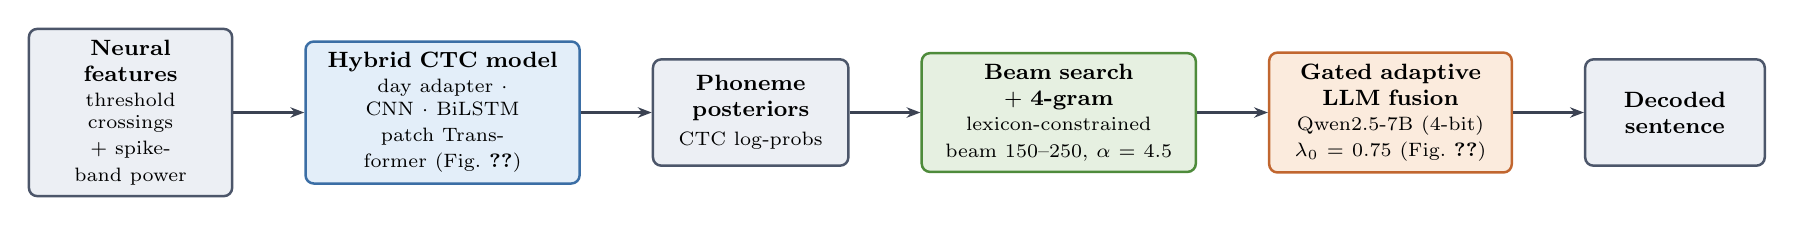
\begin{tikzpicture}[node distance=9mm]
  \node[io,minimum height=13.5mm,text width=23mm] (in)
       {\textbf{Neural}\\\textbf{features}\\[1pt]\scriptsize threshold crossings\\+ spike-band power};
  \node[ac,right=of in,minimum height=13.5mm,text width=32mm] (am)
       {\textbf{Hybrid CTC model}\\[1pt]
        \scriptsize day adapter $\cdot$ CNN $\cdot$ BiLSTM\\ patch Transformer (Fig.~\ref{fig:arch})};
  \node[io,right=of am,minimum height=13.5mm,text width=22mm] (post)
       {\textbf{Phoneme}\\\textbf{posteriors}\\[1pt]\scriptsize CTC log-probs};
  \node[de,right=of post,minimum height=13.5mm,text width=32mm] (beam)
       {\textbf{Beam search $+$ 4-gram}\\[1pt]
        \scriptsize lexicon-constrained\\ beam $150$--$250$, $\alpha=4.5$};
  \node[ll,right=of beam,minimum height=13.5mm,text width=28mm] (llm)
       {\textbf{Gated adaptive}\\\textbf{LLM fusion}\\[1pt]
        \scriptsize Qwen2.5-7B (4-bit)\\ $\lambda_0=0.75$ (Fig.~\ref{fig:fusion})};
  \node[io,right=of llm,minimum height=13.5mm,text width=20mm] (out)
       {\textbf{Decoded}\\\textbf{sentence}};

  \draw[fl] (in) -- (am); \draw[fl] (am) -- (post);
  \draw[fl] (post) -- (beam); \draw[fl] (beam) -- (llm); \draw[fl] (llm) -- (out);
\end{tikzpicture}}
\caption{End-to-end decoding pipeline. Binned neural features become phoneme posteriors under the hybrid CTC model, are expanded into an $N$-best list by a lexicon-constrained beam search with a 4-gram KenLM, and are reranked by a gated, margin-adaptive fusion of decoder and LLM scores. Only the last stage uses a large language model; at the OP-A setting shown it fires on 72\pct{} of utterances, at OP-B on 68\pct{}.}
\label{fig:pipeline}
\end{figure*}

\begin{abstract}
Intracortical speech neuroprostheses turn cortical activity into text. We describe a three-stage brain-to-text decoder for the Brain-to-Text '25 corpus
(participant T15). A 28.8\,M-parameter hybrid CNN--BiLSTM--Transformer is trained
with connectionist temporal classification over 41 phonemes; a
lexicon-constrained beam search with a 4-gram KenLM produces an $N$-best list;
and a \emph{gated, margin-adaptive} score-fusion stage lets a 4-bit quantized
large language model (LLM) rescore it. A two-sided confidence gate skips the LLM
on collapsed and on already-resolved lattices, and inside the gate the fusion
weight decays to zero with the top-1/top-2 margin. On the 1{,}426-sentence
validation split, fusion with Qwen2.5-7B moves word error rate (WER) from
7.37\pct{} to 7.26\pct{} and character error rate from 5.33\pct{} to 5.18\pct{}
while calling the LLM on \ifRvReady\RvOursCalls\else 72\fi\pct{} of utterances. \ifRvReady\ifRvSig A paired bootstrap
places the WER change at \RvDWER{} points (95\pct{} CI [\RvCIlo, \RvCIhi]).\else
A paired bootstrap shows the WER change is within noise (95\pct{} CI
[\RvCIlo, \RvCIhi] points).\fi\else A paired bootstrap gives a 95\pct{} CI of
[\RvCIlo, \RvCIhi] points for the WER change.\fi{} \ifRvCERSig The CER change is
significant ($p=\RvPc$).\fi{} On identical $N$-best lists, a constant weight on
standardized scores never helps, and under session-disjoint calibration no rule
beats the decoder alone; ours comes closest among the LLM rules while calling
the LLM on \RvOursCalls\pct{} rather than \RvUngRawCalls\pct{} of utterances. A 132-point sweep shows the optimal fusion weight shrinking as the
$n$-gram decoder strengthens: the two language priors substitute rather than
add.
\end{abstract}

\begin{IEEEkeywords}
brain--computer interface, speech neuroprosthesis, CTC, Transformer, $N$-best rescoring, large language models, score fusion
\end{IEEEkeywords}

%=======================================================================
\section{Introduction}
%=======================================================================
Amyotrophic lateral sclerosis (ALS), brainstem stroke and spinal-cord injury can
take away speech. Intracortical brain--computer interfaces (BCIs) restore part of
it, decoding attempted-speech
activity from the ventral precentral gyrus into text
\cite{willett2023speech,card2024accurate,metzger2023avatar}; recent systems also
synthesize the intended voice with sub-second delay \cite{wairagkar2025voice,littlejohn2025streaming}
and read out inner speech from the same motor-cortex arrays \cite{kunz2025inner}.
The usual text pipeline comes from automatic speech recognition (ASR): a network
maps binned multi-unit activity to phoneme posteriors under a connectionist
temporal classification (CTC) objective \cite{graves2006ctc}, a
lexicon-constrained beam search with an $n$-gram model turns those into word
hypotheses, and a neural language model optionally rescores the $N$-best list
(Fig.~\ref{fig:pipeline}).

Two observations motivate this work. The acoustic and language stages fail in
different regimes: phoneme error rate (PER) is fixed by the acoustic model and
floors everything downstream, while WER moves a great deal with how much
linguistic prior is injected during decoding. And injecting that prior uniformly
wastes computation and sometimes does damage, since a rescorer applied everywhere
will occasionally overturn a correct top-1 hypothesis and, on a collapsed
lattice, can only pick the most fluent wrong sentence. Both cases are visible in
the $N$-best scores alone, as a very low top-1 score or a wide top-1/top-2
margin. We therefore make the strength of LLM intervention a per-utterance
quantity read off the decoder's own scores, with no reference transcripts and no
fine-tuning:

\begin{itemize}
\item A hybrid CNN--BiLSTM--Transformer CTC acoustic model with per-session
adapters tied by a day-to-day \emph{drift penalty} (Section~\ref{sec:model}).
\item A two-sided confidence gate paired with a closed-form per-utterance weight
$\lambda(\mathcal{H})$ that decays to zero exactly at the gate boundary
(Section~\ref{sec:fusion}, Algorithm~\ref{alg:fusion}), so the rule is
continuous in the decoder scores.
\item A paired comparison on identical $N$-best lists with ungated, one-sided
and hard-gated fusion, using session-disjoint calibration, bootstrap intervals,
held-out test scores and latency (Section~\ref{subsec:paired}).
\item A 132-point joint sweep of the $n$-gram and fusion weights for five
open-weight rescorers, showing that the two language priors are
\emph{substitutes}: the optimal fusion weight falls from 2.50 to 0 as the
$n$-gram weight rises (Section~\ref{subsec:subst}).
\end{itemize}

Section~\ref{sec:related} reviews related work, Sections~\ref{sec:data}--\ref{sec:fusion}
cover data, acoustic model, beam search and fusion rule, Sections~\ref{sec:setup}
and \ref{sec:results} the protocol and results, and Section~\ref{sec:disc} the
implications and limits.

\begin{figure*}[!t]
\centering
\adjustbox{max width=\textwidth}{%
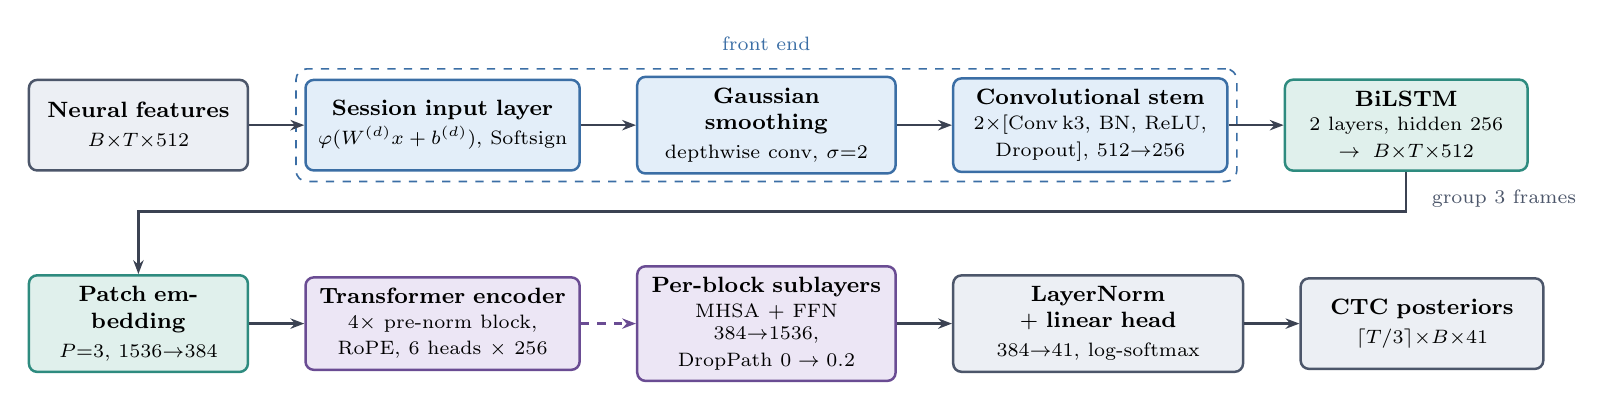
\begin{tikzpicture}[node distance=7mm]
  % ---------- row 1 ----------
  \node[io,minimum height=11.5mm,text width=25mm] (in)
       {\textbf{Neural features}\\[1pt]\scriptsize $B{\times}T{\times}512$};
  \node[ac,right=of in,minimum height=11.5mm,text width=32mm] (day)
       {\textbf{Session input layer}\\[1pt]\scriptsize $\varphi(W^{(d)}x+b^{(d)})$, Softsign};
  \node[ac,right=of day,minimum height=11.5mm,text width=30mm] (gau)
       {\textbf{Gaussian smoothing}\\[1pt]\scriptsize depthwise conv, $\sigma{=}2$};
  \node[ac,right=of gau,minimum height=11.5mm,text width=32mm] (cnn)
       {\textbf{Convolutional stem}\\[1pt]\scriptsize $2\times$[Conv\,k3, BN, ReLU,\\ Dropout], $512{\to}256$};
  \node[re,right=of cnn,minimum height=11.5mm,text width=28mm] (lstm)
       {\textbf{BiLSTM}\\[1pt]\scriptsize 2 layers, hidden 256\\ $\to B{\times}T{\times}512$};

  \foreach \a/\b in {in/day,day/gau,gau/cnn,cnn/lstm} \draw[fl] (\a) -- (\b);

  % ---------- row 2 ----------
  \node[re,below=13mm of in,minimum height=11.5mm,text width=25mm] (patch)
       {\textbf{Patch embedding}\\[1pt]\scriptsize $P{=}3$, $1536{\to}384$};
  \node[tr,right=of patch,minimum height=11.5mm,text width=32mm] (enc)
       {\textbf{Transformer encoder}\\[1pt]\scriptsize $4\times$ pre-norm block,\\ RoPE, 6 heads $\times$ 256};
  \node[tr,right=of enc,minimum height=11.5mm,text width=30mm] (ffn)
       {\textbf{Per-block sublayers}\\[1pt]\scriptsize MHSA $+$ FFN $384{\to}1536$,\\ DropPath $0\!\to\!0.2$};
  \node[io,right=of ffn,minimum height=11.5mm,text width=34mm] (head)
       {\textbf{LayerNorm $+$ linear head}\\[1pt]\scriptsize $384{\to}41$, log-softmax};
  \node[io,right=of head,minimum height=11.5mm,text width=28mm] (out)
       {\textbf{CTC posteriors}\\[1pt]\scriptsize $\lceil T/3\rceil{\times}B{\times}41$};

  \draw[fl] (patch) -- (enc);
  \draw[trLine,line width=0.9pt,dashed,-{Stealth[length=5pt]}] (enc) -- (ffn);
  \draw[fl] (ffn) -- (head); \draw[fl] (head) -- (out);

  % wrap arrow from row 1 to row 2
  \draw[fl] (lstm.south) -- ++(0,-5mm) -| (patch.north);
  \node[capt,anchor=west] at ($(lstm.south)+(2mm,-3.4mm)$)
       {\scriptsize group 3 frames};

  \begin{scope}[on background layer]
    \node[draw=acLine,dashed,rounded corners,line width=0.6pt,fit=(day)(cnn),
          inner sep=3pt] (fe) {};
  \end{scope}
  \node[capt,text=acLine,above=1mm of fe.north] {\scriptsize front end};
\end{tikzpicture}}
\caption{Hybrid CTC acoustic model (28.8\,M parameters, 10.8\,M of them in the 41 session adapters). Recurrence precedes attention: the BiLSTM integrates 20\,ms bins locally, then patches of three frames shorten the sequence threefold before four pre-norm Transformer blocks with rotary attention. Only the session input layer carries per-session parameters, regularized by the drift penalty of Eq.~(2).}
\label{fig:arch}
\end{figure*}

%=======================================================================
\section{Related Work}\label{sec:related}
%=======================================================================
\textbf{Speech neuroprostheses.} Willett \textit{et al.} \cite{willett2023speech}
demonstrated a 62 word/min speech BCI using a recurrent phoneme decoder with
$n$-gram and neural language-model rescoring. Metzger \textit{et al.}
\cite{metzger2023avatar} reported a comparable electrocorticography system, and
Card \textit{et al.} \cite{card2024accurate} cut calibration to a single session
on the 256-electrode T15 participant whose recordings form the Brain-to-Text '25
corpus \cite{kaggle2025b2t} used here. In the '24 benchmark, ensembling and
language-model rescoring produced most of the gains \cite{willett2024benchmark}.
Pretrained encoders have since advanced the acoustic side: BIT leads both
benchmarks in a cascaded setting and cuts end-to-end WER from 24.69\pct{} to
10.22\pct{} \cite{zhang2026bit}, and BrainWhisperer transfers a large ASR
model to these recordings \cite{boccato2026brainwhisperer}.
Session drift has been handled with affine transforms shared across days and
participants \cite{boccato2026crosssubject}, of which our drift penalty
\eqref{eq:drift} is the cheap version. Our acoustic model is deliberately
modest; the question here is the language stage.

\textbf{Neural rescoring.} Combining a decoder with an external language model
by log-linear interpolation, known as shallow fusion, is standard in ASR
\cite{kannan2018shallow}; masked-LM pseudo-log-likelihood scoring improves
$N$-best rescoring without retraining the acoustic model
\cite{salazar2020mlmscoring}, and sequence-to-sequence error correction over
multiple hypotheses \cite{ma2023nbestt5,chen2023hyporadise} carries the idea into generation. Two
BCI systems sit closest to our stage: Li \textit{et al.} \cite{li2025dcond} have
an LLM select and merge among decoder hypotheses on the '24 corpus, reaching
5.77\pct{} WER with a fine-tuned model, and Olak \textit{et al.}
\cite{olak2026decoding} pair contextual sequence-to-sequence decoding with
phoneme readout, finding word-level accuracy competitive rather than leading.
Generative correction can quietly repair a disfluent but correct verbatim
transcript, so we keep the LLM in a pure scoring role.

\textbf{What is new here.} Almost every rescorer above runs on every hypothesis
list under one global interpolation weight. Deciding \emph{whether} to trust a
hypothesis from the $N$-best scores is itself old: top-1/top-2 margins and
posteriors are standard ASR confidence measures \cite{jiang2005confidence}. The
one gated rescorer we know of on this corpus is a Brain-to-Text '25 competition
entry \cite{cheng2026kaggle7}, which switches Mistral-7B rescoring on only when
a normalized $n$-gram score clears a fixed threshold, so we claim no priority
over gating itself. What we add is (i) a \emph{two-sided} gate that also
withholds the LLM where the decoder is already decisive, not only where it has
collapsed; (ii) a closed-form fusion weight in the top-1/top-2 margin, vanishing
exactly at the gate, which makes the rescorer a continuous strict superset of the
baseline rather than a hard switch; and (iii) per-list $z$-standardization in
place of a tuned temperature. Section~\ref{subsec:paired} tests each one.

%=======================================================================
\section{Data and Preprocessing}\label{sec:data}
%=======================================================================
We use the Brain-to-Text '25 corpus recorded from participant T15, who has ALS
and severe dysarthria and is implanted with four 64-channel microelectrode arrays
(256 electrodes) in left ventral precentral gyrus \cite{card2024accurate}. Each
trial gives a $T\times512$ feature matrix: per electrode, a binned
threshold-crossing count and a spike-band power estimate at 20\,ms resolution.
Labels come as sentence text and as phoneme sequences over 41 symbols (39 ARPAbet
phonemes, a CTC blank, a word boundary). The validation split has 1{,}426
sentences and the held-out test split 1{,}450, whose labels are hidden and
scored only by the competition server \cite{kaggle2025b2t}.

Per-channel statistics, accumulated over the training split with Welford's
algorithm, are reused unchanged for validation and test. Features are $z$-scored and
clipped to $\pm5$. During training only, an augmentation operator fires with
probability $0.5$, composing piecewise-linear time warping with factor
$\sim\mathcal{U}(0.9,1.1)$ ($p{=}0.3$), Gaussian noise with
$\sigma\sim\mathcal{U}(0.01,0.05)$ ($p{=}0.3$), and zeroing of a random
10\pct{} of channels ($p{=}0.2$), which guards against the electrode loss
that array drift produces \cite{sussillo2016robust}.

\begin{figure*}[!t]
\centering
\adjustbox{max width=0.98\textwidth}{%
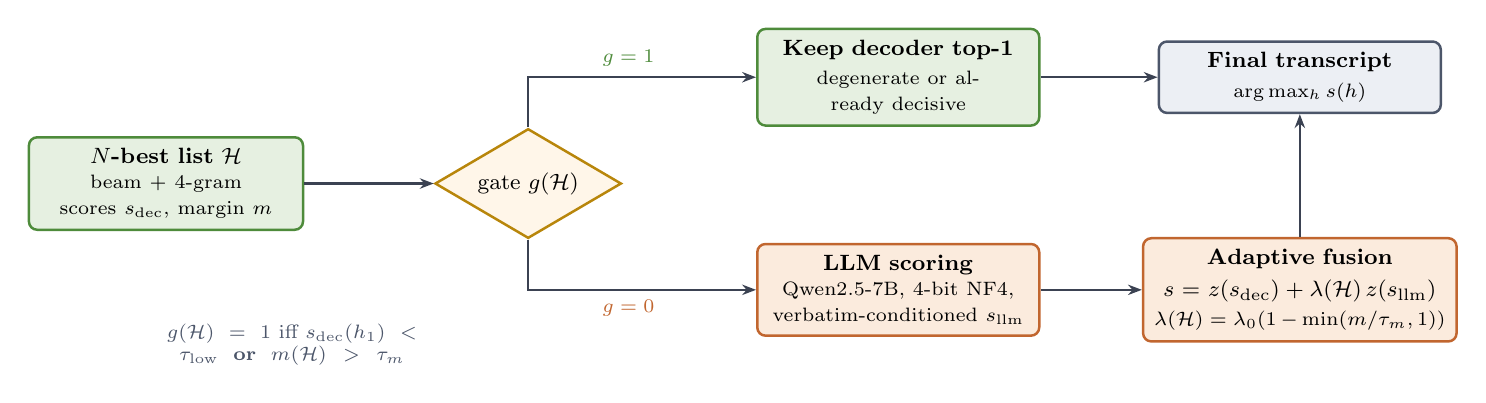
\begin{tikzpicture}[every node/.style={font=\footnotesize}]
  \node[de,text width=32mm] (nb) at (0,0)
       {\textbf{$N$-best list $\mathcal{H}$}\\[1pt]\scriptsize beam $+$ 4-gram\\ scores $s_{\mathrm{dec}}$, margin $m$};
  \node[gate,text width=17mm] (g) at (4.6,0) {gate $g(\mathcal{H})$};
  \node[de,text width=33mm] (keep)  at (9.3,1.35)
       {\textbf{Keep decoder top-1}\\[1pt]\scriptsize degenerate or already decisive};
  \node[ll,text width=33mm] (score) at (9.3,-1.35)
       {\textbf{LLM scoring}\\[1pt]\scriptsize Qwen2.5-7B, 4-bit NF4,\\ verbatim-conditioned $s_{\mathrm{llm}}$};
  \node[ll,text width=37mm] (fuse) at (14.4,-1.35)
       {\textbf{Adaptive fusion}\\[2pt]
        $s=z(s_{\mathrm{dec}})+\lambda(\mathcal{H})\,z(s_{\mathrm{llm}})$\\[1pt]
        \scriptsize $\lambda(\mathcal{H})=\lambda_0(1-\min(m/\tau_m,1))$};
  \node[io,text width=33mm] (out) at (14.4,1.35)
       {\textbf{Final transcript}\\[1pt]\scriptsize $\arg\max_h s(h)$};

  \draw[fl] (nb) -- (g);
  \draw[fl] (g) |- node[capt,pos=0.72,above,text=deLine]{$g=1$} (keep);
  \draw[fl] (g) |- node[capt,pos=0.72,below,text=llLine]{$g=0$} (score);
  \draw[fl] (score) -- (fuse);
  \draw[fl] (fuse) -- (out);
  \draw[fl] (keep) -- (out);

  \node[capt,text width=46mm,align=center] at (1.6,-2.05)
       {$g(\mathcal{H})=1$ iff $s_{\mathrm{dec}}(h_1)<\tau_{\mathrm{low}}$ \textbf{ or } $m(\mathcal{H})>\tau_m$};
\end{tikzpicture}}
\caption{Gated, margin-adaptive score fusion. The two-sided gate withholds the LLM from degenerate lattices ($s_{\text{dec}}(h_1)<\tau_{\text{low}}$, bottom 1\pct{}) and from those the decoder has resolved ($m>\tau_m$, top quartile). On the rest, the weight decays linearly with the margin, reaching zero at the gate so the decision rule stays continuous.}
\label{fig:fusion}
\end{figure*}

%=======================================================================
\section{Hybrid Acoustic Model}\label{sec:model}
%=======================================================================
The model (Fig.~\ref{fig:arch}) maps $x\in\mathbb{R}^{B\times T\times512}$ and a
session index $d$ to phoneme log-posteriors. Equations~\eqref{eq:drift}, \eqref{eq:gate},
\eqref{eq:lambda} and \eqref{eq:decision} are ours; the others restate the cited
sources in our notation.

\subsection{Session-specific input layer and drift penalty}
Recordings are non-stationary across days, so following the day-specific input
transform of \cite{willett2023speech} each session $d$ owns a full-rank affine
map, squashed by the Softsign nonlinearity of \cite{glorot2010understanding}:
\begin{equation}\label{eq:adapter}
\tilde{x}_t^{(d)}=\varphi\!\left(W^{(d)}x_t+b^{(d)}\right),\qquad
\varphi(u)=\frac{u}{1+|u|},
\end{equation}
with $W^{(d)}\in\mathbb{R}^{512\times512}$ initialized to the identity and
$b^{(d)}=0$. These adapters hold 10.8\,M of the 28.8\,M parameters, so left
alone they overfit sessions with few trials. A drift penalty ties adjacent
sessions,
\begin{equation}\label{eq:drift}
\mathcal{L}_{\text{drift}}=\frac{1}{D-1}\sum_{d=1}^{D-1}
\Big(\big\|W^{(d)}-W^{(d-1)}\big\|_F^2+\big\|b^{(d)}-b^{(d-1)}\big\|_2^2\Big),
\end{equation}
so the objective is
$\mathcal{L}=\mathcal{L}_{\text{CTC}}+\lambda_{\text{drift}}\mathcal{L}_{\text{drift}}$
with $\lambda_{\text{drift}}=0.01$: a first-order smoothness prior over the
session axis, allowing gradual drift but penalizing abrupt per-session solutions.

\subsection{Smoothing, convolutional stem and recurrent core}
A fixed Gaussian kernel ($\sigma=2$ bins, truncated at an absolute value of
$0.01$ and renormalized) runs as a depthwise temporal convolution. Two
convolutional blocks (kernel 3; batch norm; ReLU; dropout $0.2$) project
$512\rightarrow256\rightarrow256$ channels, and a two-layer bidirectional LSTM
with 256 units per direction (dropout 0.4 elsewhere in the network) gives a 512-dimensional sequence, packed by true
length.

\subsection{Patch embedding and Transformer encoder}
Keeping the recurrence \emph{before} the attention lets the Transformer
\cite{vaswani2017attention} run on a three-fold-downsampled patch sequence,
cutting attention cost by $9\times$. Groups of $P=3$ frames are concatenated and
projected, $\mathrm{LN}\rightarrow\mathrm{Linear}(1536\rightarrow384)
\rightarrow\mathrm{LN}\rightarrow\mathrm{Dropout}$. Four pre-norm residual blocks
\cite{xiong2020prenorm} follow,
\begin{align}
z &\leftarrow z+\mathrm{DropPath}_{p_\ell}\!\big(\mathrm{MHSA}_{\text{RoPE}}(\mathrm{LN}(z))\big),\label{eq:attn}\\
z &\leftarrow z+\mathrm{DropPath}_{p_\ell}\!\big(\mathrm{FFN}(\mathrm{LN}(z))\big),\label{eq:ffn}
\end{align}
with stochastic-depth rate $p_\ell$ rising linearly from $0$ to $0.2$
\cite{huang2016stochastic}. Attention is deliberately \emph{wide rather than
deep}: 6 heads of dimension 256 (inner width 1536, four times
$d_{\text{model}}=384$), rotary embeddings \cite{su2024roformer} and attention
dropout $0.5$. The feed-forward block is $384\rightarrow1536\rightarrow384$ with
GELU, and a final LayerNorm plus linear head gives 41 logits per patch whose
log-softmax feeds CTC \cite{graves2006ctc}.

\subsection{Optimization}
AdamW (learning rate $5\times10^{-4}$, weight decay $10^{-4}$) runs one-cycle
cosine annealing with a 10\pct{} warm-up over 82 epochs at batch size 16, with
mixed precision and gradient-norm clipping at 5.0. Training stops after 10
epochs without improvement in validation WER; the three best checkpoints are
averaged in weight space \cite{izmailov2018swa}; that model produced every
reported number.

%=======================================================================
\section{Lexicon-Constrained Beam Search}\label{sec:beam}
%=======================================================================
Emissions are decoded by a lexicon-constrained CTC beam search (Flashlight
\cite{kahn2022flashlight} through \texttt{torchaudio}) with a 4-gram KenLM
\cite{heafield2011kenlm} estimated on a mixed Wikipedia, news and Switchboard
corpus. Only hypotheses whose phoneme paths match the pronunciation-lexicon trie
survive, so every token is a real word. A hypothesis $h$ with words $w_{1:M}$ is
scored by the usual log-linear combination of acoustic and language-model scores
\cite{willett2023speech,kannan2018shallow},
\begin{equation}\label{eq:beam}
S(h)=\log p_{\text{AM}}(h)+\alpha\log p_{\text{4gram}}(w_{1:M})+\beta M ,
\end{equation}
with $n$-gram weight $\alpha$ and word insertion bonus $\beta$, fixed at $0$ and
not tuned. Downstream comparisons use the length-normalized score
$s_{\text{dec}}(h)=S(h)/\max(M,1)$. Our main configuration is beam 250 with
30-best; with no LLM it reaches 7.55\pct{} WER at $\alpha=4.5$ and 7.37\pct{}
at $\alpha=5.5$, a 0.18-point gap that decides most of what rescoring can add.

%=======================================================================
\section{Gated, Margin-Adaptive LLM Score Fusion}\label{sec:fusion}
%=======================================================================
Let $\mathcal{H}=(h_1,\dots,h_N)$ be the $N$-best list of one utterance, ordered
by $s_{\text{dec}}$. Fig.~\ref{fig:fusion} sketches the stage and
Algorithm~\ref{alg:fusion} states it exactly.

\subsection{Verbatim-conditioned LLM scoring}
A causal LM $p_\theta$ in 4-bit NF4 \cite{dettmers2023qlora} runs in scoring
mode only. Each hypothesis $t(h)=(t_1,\dots,t_L)$ follows a fixed instruction $c$
stating that the text is a raw, word-for-word transcript that may contain false
starts; $c$ is masked out of the length-normalized log-likelihood used for LM
rescoring \cite{salazar2020mlmscoring}:
\begin{equation}\label{eq:llm}
s_{\text{llm}}(h)=\frac{1}{L}\sum_{i=1}^{L}\log p_\theta\!\left(t_i \mid c, t_{<i}\right).
\end{equation}
Without $c$, a well-aligned LLM prefers the grammatically tidier candidate, the
wrong prior for verbatim speech. All $N$ hypotheses are scored in one batch, so
the LLM costs one forward pass per utterance.

\subsection{Two-sided confidence gate}
The LLM helps only in a middle band of decoder confidence. With the top-1/top-2
margin $m(\mathcal{H})=s_{\text{dec}}(h_1)-s_{\text{dec}}(h_2)$, a classic
$N$-best confidence measure \cite{jiang2005confidence} ($m=\infty$ when $N<2$),
two thresholds are taken from the empirical distribution over a calibration set
$\mathcal{U}$, using no transcripts:
\begin{equation}\label{eq:thresh}
\tau_{\text{low}}=Q_{1}\big(\{s_{\text{dec}}(h_1^{(u)})\}_{u\in\mathcal{U}}\big),\quad
\tau_{m}=Q_{75}\big(\{m(\mathcal{H}^{(u)})\}_{u\in\mathcal{U}}\big),
\end{equation}
where $Q_q$ is the $q$-th percentile. The gate is
\begin{equation}\label{eq:gate}
g(\mathcal{H})=\mathbb{1}\big[s_{\text{dec}}(h_1)<\tau_{\text{low}}\big]\;\vee\;\mathbb{1}\big[m(\mathcal{H})>\tau_{m}\big].
\end{equation}
The first clause drops the bottom 1\pct{}, where the signal has collapsed and a
fluency prior can only pick a more plausible-sounding error. The second drops the
top quartile by margin, where reordering is likelier to break a correct answer
than fix a wrong one.

\subsection{Adaptive fusion weight and decision rule}
Inside the gate the weight decays linearly with the margin,
\begin{equation}\label{eq:lambda}
\lambda(\mathcal{H})=\lambda_0\left(1-\min\!\left(\frac{m(\mathcal{H})}{\tau_m},1\right)\right),
\end{equation}
so it vanishes exactly where the gate switches and utterances just inside and
just outside receive the same transcript. Writing $z(\cdot)$ for the $z$-score
over the current list ($z\equiv0$ if its standard deviation is below
$10^{-8}$), the fused score and transcript are
\begin{align}
s(h) &= z\big(s_{\text{dec}}(h)\big)+\lambda(\mathcal{H})\,z\big(s_{\text{llm}}(h)\big),\label{eq:fused}\\
\hat{y} &=
\begin{cases}
h_1, & g(\mathcal{H})=1 \ \text{or}\ \lambda(\mathcal{H})=0,\\[2pt]
\arg\max_{h\in\mathcal{H}} s(h), & \text{otherwise.}
\end{cases}\label{eq:decision}
\end{align}
Equation~\eqref{eq:fused} is shallow fusion \cite{kannan2018shallow} with
per-list standardization in place of a tuned temperature, so $\lambda_0$ means
the same for a short confident utterance and a long ambiguous one. Setting
$\lambda_0=0$ reproduces the beam$+n$-gram decoder exactly, so the stage is a
strict superset of the baseline.

\subsection{Calibration protocol for unseen data}\label{subsec:calib}
The thresholds need no transcripts, but where they are estimated matters.
Throughout, $\tau_{\text{low}}$, $\tau_m$ and $\lambda_0$ are fitted on labelled
validation data and frozen; no statistic is computed on test data.
Section~\ref{subsec:paired} also fits all three on half of the validation
sessions and applies them to the other half. For a new session or streaming use we
recommend the same freeze-then-apply rule: calibrate on the first labelled
block, or track the two percentiles online with the P$^2$ estimator
\cite{jain1985p2}, which updates a quantile in constant memory per utterance.

\begin{algorithm}[!t]
\caption{Gated, margin-adaptive LLM score fusion}
\label{alg:fusion}
\footnotesize
\begin{algorithmic}[1]
\Require $N$-best lists $\{\mathcal{H}^{(u)}\}_{u\in\mathcal{U}}$, scores
         $s_{\text{dec}}$, base weight $\lambda_0$, percentiles $q_s{=}1$,
         $q_m{=}75$, LM $p_\theta$, verbatim prefix $c$
\Statex \textit{Stage 1 -- gate calibration, no reference transcripts}
\ForAll{nonempty $\mathcal{H}^{(u)}$}
  $\sigma_u \!\gets\! s_{\text{dec}}(h_1^{(u)})$,
  $m_u \!\gets\! \sigma_u\!-\!s_{\text{dec}}(h_2^{(u)})$ ($\infty$ if $N_u{<}2$)
\EndFor
\State $\tau_{\text{low}} \gets Q_{q_s}(\{\sigma_u\})$,\quad
       $\tau_m \gets Q_{q_m}(\{m_u : m_u<\infty\})$
\Statex \textit{Stage 2 -- gated fusion}
\ForAll{$u \in \mathcal{U}$}
  \If{$\sigma_u<\tau_{\text{low}}$ \textbf{or} $m_u>\tau_m$}
     \State $\hat{y}^{(u)} \gets h_1^{(u)}$ \Comment{gate fires; LLM unused}
  \Else
     \State $\lambda_u \gets \lambda_0\big(1-\min(m_u/\tau_m,\,1)\big)$
     \State $\{s_{\text{llm}}(h)\} \gets p_\theta(\cdot \mid c)$ over
            $\mathcal{H}^{(u)}$ \Comment{one batched pass}
     \State $\hat{y}^{(u)} \gets \arg\max_{h}
            z(s_{\text{dec}}(h))+\lambda_u z(s_{\text{llm}}(h))$
  \EndIf
\EndFor
\State \textbf{return} $\{\hat{y}^{(u)}\}$ \ ($\varepsilon$ for empty lists)
\end{algorithmic}
\end{algorithm}

%=======================================================================
\section{Experimental Setup}\label{sec:setup}
%=======================================================================
Hypotheses and references pass through the official text normalization before
corpus-level WER and CER. PER is the Levenshtein distance between greedy CTC
output and ground-truth phonemes, so it depends only on the acoustic model.
Two operating points recur below, both with beam 250, 30-best, Qwen2.5-7B and
gate percentiles 1/75: OP-A ($\alpha=4.5$, $\lambda_0=0.75$,
$\tau_{\text{low}}=-28.45$, $\tau_m=5.36$) and the joint grid optimum OP-B
($\alpha=5.5$, $\lambda_0=1.25$, $\tau_{\text{low}}=-32.15$, $\tau_m=6.10$).

\textbf{Rescorers.} Five open-weight LLMs share 4-bit quantization and scoring
code: Qwen2.5-7B \cite{qwen2024qwen25}, Qwen3-4B, Mistral-7B
\cite{jiang2023mistral}, Llama-3.2-3B-Instruct \cite{grattafiori2024llama3}
and Gemma-3-4B \cite{gemma2025gemma3}, each at its own best
$(\alpha,\lambda_0)$ and against the $\lambda_0{=}0$ baseline of its own beam
configuration (250 for Qwen and Llama, an earlier 150 for Mistral and Gemma).

\textbf{Paired comparison.} On the OP-B lists the LLM scores every hypothesis
once and six rules reuse those scores:
ungated shallow fusion with raw scores, the same with per-list $z$-scores, a
one-sided gate (the first clause of \eqref{eq:gate} alone, as in
\cite{cheng2026kaggle7}), a hard two-sided gate with constant $\lambda_0$, the
adaptive weight \eqref{eq:lambda} without the gate, and ours. Each rule gets its
best weight from the same grid, fitted on all validation data or, in the
session-disjoint mode, with its thresholds on a random half of the sessions and
applied to the other half, and vice versa.

\textbf{Statistics and cost.} Differences are tested with a paired bootstrap
\cite{bisani2004bootstrap} ($10^4$ resamples) over utterances and, to respect
within-session correlation, over whole sessions, plus an exact sign test on
per-utterance word-error changes; a 95\pct{} interval that contains zero is
reported as a tie. Latency is wall-clock time per utterance on one NVIDIA T4
(16\,GB): the beam search takes \RvTdec\,ms and one batched LLM pass over a 30-best
list \RvTllm\,s (median \RvTllmMed\,s). The 132-point grid took 7.6\,h.


%=======================================================================
\section{Results and Analysis}\label{sec:results}
%=======================================================================

\subsection{Main result and rescorer comparison}
At OP-B gated adaptive fusion reaches 7.26\pct{} WER and
5.18\pct{} CER against a 7.37\pct{} / 5.33\pct{} $n$-gram baseline at the same
$\alpha$. At OP-A fusion leaves
WER at 7.55\pct{} and still cuts CER from 5.38\pct{} to 5.31\pct{}, a first sign
that the two stages compete for the same errors. PER is 12.12\pct{} throughout.

In Table~\ref{tab:llms} accuracy does not follow parameter count: Llama-3.2-3B
finishes within 0.07 WER points of the 7\,B Qwen2.5, with the lowest CER of any
run. Against a well-tuned decoder the WER gain is 0.00 to 0.11 points; CER gains
are larger because reordering usually swaps one word for a phonetic neighbour. A
poorly matched rescorer is neutralized rather than harmful: for Gemma-3-4B and
Qwen3-4B the sweep chose $\lambda_0=0$, which by \eqref{eq:decision}
reproduces the baseline exactly.

\begin{table}[!t]
\centering
\caption{Validation results for five open-weight rescorers (1{,}426 sentences), each at its own best $(\alpha,\lambda_0)$. Baselines are the $\lambda_0{=}0$ decoder of the same beam configuration. PER equals 12.12\pct{} throughout.}
\label{tab:llms}
\footnotesize
\setlength{\tabcolsep}{4pt}
\begin{tabular}{@{}lccccc@{}}
\toprule
\textbf{Rescoring LLM} & $\alpha$ & $\lambda_0$ &
\textbf{WER (\%)} & \textbf{CER (\%)} & $\Delta$\textbf{WER}\\
 & & & base\,$\to$\,fused & base\,$\to$\,fused & \\
\midrule
\multicolumn{6}{@{}l}{\itshape Wide decoder (beam 250, 30-best), baseline 7.37\pct{} WER}\\
Qwen2.5-7B        & 5.5 & 1.25 & 7.37 $\to$ \textbf{7.26} & 5.33 $\to$ 5.18 & $-0.11$\\
Llama-3.2-3B-It   & 5.5 & 0.50 & 7.37 $\to$ 7.33 & 5.33 $\to$ \textbf{5.16} & $-0.04$\\
Qwen3-4B          & 5.5 & 0.00 & 7.37 $\to$ 7.37 & 5.33 $\to$ 5.33 & $\phantom{-}0.00$\\
\addlinespace[2pt]
\multicolumn{6}{@{}l}{\itshape Narrow decoder (beam 150, 30-best), baseline 8.33\pct{} WER}\\
Mistral-7B        & 4.0 & 0.50 & 8.33 $\to$ 8.27 & 5.87 $\to$ 5.75 & $-0.06$\\
Gemma-3-4B        & 4.0 & 0.00 & 8.33 $\to$ 8.33 & 5.87 $\to$ 5.87 & $\phantom{-}0.00$\\
\bottomrule
\end{tabular}
\end{table}

\subsection{Paired comparison with existing rescoring rules}\label{subsec:paired}
Table~\ref{tab:paired} applies seven rules to identical OP-B lists. \ifRvSig
Against the baseline, ours changes WER by \RvDWER{} points (95\pct{} CI
[\RvCIlo, \RvCIhi], $p=\RvPw$); the session-level bootstrap gives
[\RvSessCIlo, \RvSessCIhi], so the gain survives within-session correlation.
\else Against the baseline, ours changes WER by \RvDWER{} points, but the
95\pct{} interval [\RvCIlo, \RvCIhi] ($p=\RvPw$; session-level
[\RvSessCIlo, \RvSessCIhi]) contains zero, so on WER alone the gain is a tie.
\fi{} \ifRvCERSig The CER change, \RvDCER{} points
([\RvCERCIlo, \RvCERCIhi], $p=\RvPc$), is significant at this operating
point. \else The CER change,
\RvDCER{} points ([\RvCERCIlo, \RvCERCIhi], $p=\RvPc$), is likewise within
noise. \fi{} Per utterance the rule improves \RvUttBetter{} transcripts and
worsens \RvUttWorse{} (sign test $p=\RvPsign$); per session it helps
\RvSessBetter{} and hurts \RvSessWorse{} of \RvNsess.

Session-disjoint calibration is the inductive check, and it removes the gain.
Fitting thresholds and $\lambda_0$ on the other half of the sessions moves our
WER from \RvOursWER\pct{} to \RvOursWERcv\pct{}, \RvDWERcv{} points against
the baseline (CI [\RvCIloCV, \RvCIhiCV]), and CER to \RvOursCERcv\pct{}
against \RvBaseCERcv\pct{}. No rule beats the decoder alone under
this protocol. Ours stays closest and is the best of the six LLM rules,
\RvDWERbest{} points against the strongest, ungated fusion of raw scores (CI
[\RvCIloBest, \RvCIhiBest]), while calling the LLM on \RvOursCalls\pct{} of
utterances instead of \RvUngRawCalls\pct{}. The table also isolates the
adaptive weight: with standardized scores every constant-weight rule, gated or
not, selects $\lambda_0=0$, so the transductive gain comes from letting the
weight decay with the margin.

\begin{table}[!t]
\centering
\caption{Rescoring rules on identical OP-B validation lists (1{,}426 sentences).
$\lambda_0$: weight chosen on all validation data ($0$ disables the LLM).
LLM: share of utterances scored. Session-disjoint: thresholds and $\lambda_0$ fitted on the other half
of the sessions.}
\label{tab:paired}
\footnotesize
\setlength{\tabcolsep}{3.2pt}
\begin{tabular}{@{}lcccccc@{}}
\toprule
 & & & \multicolumn{2}{c}{\textbf{Transductive}} & \multicolumn{2}{c}{\textbf{Session-disjoint}}\\
\cmidrule(lr){4-5}\cmidrule(l){6-7}
\textbf{Rule} & $\lambda_0$ & \textbf{LLM\,\%} & \textbf{WER} & \textbf{CER} & \textbf{WER} & \textbf{CER}\\
\midrule
Beam $+$ 4-gram only    & -- & \RvBaseCalls & \RvBaseWER & \RvBaseCER & \RvBaseWERcv & \RvBaseCERcv\\
Ungated, raw scores     & \RvUngRawLam & \RvUngRawCalls & \RvUngRawWER & \RvUngRawCER & \RvUngRawWERcv & \RvUngRawCERcv\\
Ungated, $z$-scores     & \RvUngZLam & \RvUngZCalls & \RvUngZWER & \RvUngZCER & \RvUngZWERcv & \RvUngZCERcv\\
One-sided gate          & \RvOneSidedLam & \RvOneSidedCalls & \RvOneSidedWER & \RvOneSidedCER & \RvOneSidedWERcv & \RvOneSidedCERcv\\
Two-sided, hard         & \RvHardTwoLam & \RvHardTwoCalls & \RvHardTwoWER & \RvHardTwoCER & \RvHardTwoWERcv & \RvHardTwoCERcv\\
Adaptive, no gate       & \RvAdaptNoGateLam & \RvAdaptNoGateCalls & \RvAdaptNoGateWER & \RvAdaptNoGateCER & \RvAdaptNoGateWERcv & \RvAdaptNoGateCERcv\\
\textbf{Ours}           & \RvOursLam & \RvOursCalls & \RvOursWER & \RvOursCER & \RvOursWERcv & \RvOursCERcv\\
\bottomrule
\end{tabular}
\end{table}

\subsection{The two language priors substitute for one another}\label{subsec:subst}
In Fig.~\ref{fig:sweeps}, WER falls from 15.85\pct{} at $\alpha=0.5$ to
7.26\pct{} at $\alpha=5.5$ and ticks back up to 7.38\pct{} at $\alpha=6.0$, so
the optimum is interior. The fusion weight moves the other way (panel a): where
the $n$-gram prior is weak the grid picks the largest $\lambda_0=2.5$; as
$\alpha$ grows the best $\lambda_0$ falls to 1.75, 1.5, 1.25, and at
$\alpha=6.0$ to zero. Once the cheap prior is tuned, little is left for the
expensive one. Panel (b)
is the $\lambda_0$ sweep at $\alpha=5.5$: an interior WER minimum of 7.26\pct{}
at $\lambda_0=1.25$ against 7.37\pct{} at $\lambda_0=0$ and 7.60\pct{} at
$\lambda_0=2.5$, so over-trusting the LLM erodes the gain.

\begin{figure}[!t]
\centering
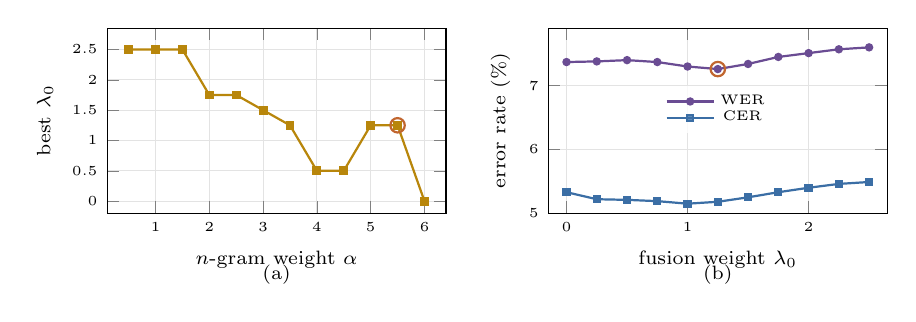
\begin{tikzpicture}
\begin{axis}[
  name=pA,
  width=0.355\columnwidth, height=2.35cm, scale only axis,
  xlabel={$n$-gram weight $\alpha$}, ylabel={best $\lambda_0$},
  xmin=0.1, xmax=6.4, ymin=-0.2, ymax=2.85,
  xtick={1,2,3,4,5,6}, ytick={0,0.5,1.0,1.5,2.0,2.5},
  yticklabel style={/pgf/number format/fixed,
                    /pgf/number format/precision=2},
  tick label style={font=\tiny}, label style={font=\scriptsize},
  grid=major, grid style={gray!22},
]
\addplot[color=gaLine,mark=square*,mark size=1.2pt,line width=0.8pt]
  coordinates {(0.5,2.50)(1.0,2.50)(1.5,2.50)(2.0,1.75)(2.5,1.75)(3.0,1.50)
               (3.5,1.25)(4.0,0.50)(4.5,0.50)(5.0,1.25)(5.5,1.25)(6.0,0.00)};
\addplot[only marks,mark=o,mark size=2.6pt,color=llLine,line width=0.8pt]
  coordinates {(5.5,1.25)};
\end{axis}

\begin{axis}[
  name=pB,
  width=0.355\columnwidth, height=2.35cm, scale only axis,
  at={($(pA.east)+(1.30cm,0)$)}, anchor=west,
  xlabel={fusion weight $\lambda_0$}, ylabel={error rate (\%)},
  xmin=-0.15, xmax=2.65, ymin=5.0, ymax=7.9,
  xtick={0,1,2}, ytick={5,6,7},
  tick label style={font=\tiny}, label style={font=\scriptsize},
  legend style={font=\tiny,at={(0.50,0.56)},anchor=center,draw=none,
                fill=white,fill opacity=0.8,text opacity=1,row sep=-3pt,
                inner sep=1pt},
  grid=major, grid style={gray!22},
]
\addplot[color=trLine,mark=*,mark size=1.1pt,line width=0.8pt]
  coordinates {(0,7.37)(0.25,7.38)(0.5,7.40)(0.75,7.37)(1.0,7.30)(1.25,7.26)
               (1.5,7.34)(1.75,7.45)(2.0,7.51)(2.25,7.57)(2.5,7.60)};
\addlegendentry{WER}
\addplot[color=acLine,mark=square*,mark size=1.1pt,line width=0.8pt]
  coordinates {(0,5.33)(0.25,5.22)(0.5,5.21)(0.75,5.19)(1.0,5.15)(1.25,5.18)
               (1.5,5.25)(1.75,5.33)(2.0,5.40)(2.25,5.46)(2.5,5.49)};
\addlegendentry{CER}
\addplot[only marks,mark=o,mark size=2.6pt,color=llLine,line width=0.8pt]
  coordinates {(1.25,7.26)};
\end{axis}
\node[font=\scriptsize] at ($(pA.south)+(0,-0.78cm)$) {(a)};
\node[font=\scriptsize] at ($(pB.south)+(0,-0.78cm)$) {(b)};
\end{tikzpicture}
\caption{Joint sweep for Qwen2.5-7B, wide decoder, 132 grid points. (a) Best
fusion weight per $n$-gram weight; it collapses from 2.50 to 0 as the $n$-gram
prior is tuned up, so the priors substitute rather than add. (b) WER and CER
against $\lambda_0$ at $\alpha=5.5$. Circles mark the grid optimum.}
\label{fig:sweeps}
\end{figure}

\subsection{Behaviour of the gate}\label{subsec:gate}
At OP-A the gate withholds the LLM from 393 of 1{,}426 utterances
(27.6\pct{}): 15 degenerate and 378 already decisive, and the mean applied
weight is $\bar{\lambda}=0.418$ against a base of $0.75$; at OP-B it is
withheld from 32\pct{}. Being percentiles, both
thresholds track the score scale on their own: $\tau_{\text{low}}$ runs from
$-12.02$ at $\alpha=0.5$ to $-34.21$ at $\alpha=6.0$ and $\tau_m$ from $0.58$ to
$6.33$ without retuning.

\subsection{Held-out test, sessions and published systems}\label{subsec:test}
On the 1{,}450-sentence test split, scored by the competition server with
thresholds and $\lambda_0$ frozen from validation, OP-B reaches 9.34\pct{} WER on
the private two-thirds and 8.21\pct{} on the public third, calling the LLM on
\RvTestCalls\pct{} of test utterances. Test transcripts are hidden, so the gain
over the decoder alone is tested on validation (Section~\ref{subsec:paired}). Per-session validation WER runs from 0.60\pct{} on
\texttt{t15.2023.12.10} to 37.04\pct{} on \texttt{t15.2025.03.14}, an ordering
set by the acoustic stage and identical across rescorers.

Protocols differ across published systems. On our validation split a phonetic
GRU reports 21.19\pct{} WER at 12.62\pct{} PER \cite{zamora2026phoneme}. On
T15 splits we cannot match trial for trial, BIT reports 10.22\pct{} WER
end-to-end \cite{zhang2026bit}, BrainWhisperer 8.7\pct{} under cross-dataset
training \cite{boccato2026brainwhisperer}, and the LLM-rescored competition
baseline 6.70\pct{} on the test split \cite{kaggle2025b2t}. We claim no state
of the art.

%=======================================================================
\section{Discussion and Limitations}\label{sec:disc}
%=======================================================================
\textbf{The priors substitute.} Tuning $\alpha$ from 4.5 to 5.5 gains more
than fusion then adds, so tuning the rescorer but not the $n$-gram weight
overstates what the LLM contributes. Our 12.12\pct{} PER trails the pretrained
encoders \cite{zhang2026bit,boccato2026brainwhisperer}; that gap, not the
rescorer, is where the headroom sits, and the fusion rule is orthogonal to it.

\textbf{What this means for a deployed BCI.} Against the decoder alone, an LLM
stage does not yet pay for itself on WER. Among ways of adding one, the gate is
the cheapest and safest: a pass costs about \RvTllm\,s against \RvTdec\,ms of
beam search, each skipped utterance saves most of that, and the rule's worst
case is the decoder itself. Verbatim conditioning
serves the same goal: a user is better served by the sentence they attempted,
false start included, than by a fluent paraphrase.

\textbf{How far it generalizes.} Across sessions, the session-disjoint check and
the 36-point per-session spread bound the claim: the rule cannot rescue a session
whose phoneme posteriors have collapsed. It reads only $N$-best and LLM scores
through percentiles that rescale on their own (Section~\ref{subsec:gate}), so it
should transfer to any phoneme decoder with a beam search. The acoustic model is less
portable: its 10.8\,M adapter parameters and drift penalty were fitted to one
participant, and the T12 recordings of the '24 benchmark
\cite{willett2024benchmark} are the natural next test.

\textbf{Limitations.} The system is offline and all results come from one
participant. Checkpoint selection and tuning used the validation split, so the
session-disjoint and test numbers are the fairer estimates. Table~\ref{tab:llms} mixes two beam configurations, so each model
is reported against its own baseline; Table~\ref{tab:paired} uses one.

%=======================================================================
\section{Conclusion}
%=======================================================================
A gated, margin-adaptive fusion rule applies a quantized LLM only where the beam
search is undecided, skips it on 28--32\pct{} of utterances, and degrades to the
pure decoder rather than to errors when the rescorer is a poor match. Calibrated
on validation, its CER gain is significant and its WER gain within noise; under
session-disjoint calibration both come within 0.02 points of the decoder alone,
because a well-tuned 4-gram decoder already supplies
most of the prior an LLM would contribute, so rescoring gains should be reported
with the decoder they were measured against. Future work will calibrate online
and move the rule onto a pretrained encoder, where the phoneme floor is lower.

\textbf{Code, data and video.} The data are public \cite{kaggle2025b2t}. Code,
pinned configurations and the paired-comparison script behind
Table~\ref{tab:paired} are at \GitHubLink{}; the trained checkpoint, lexicon,
token list and 4-gram language model are archived at \ZenodoLink{}. A
walkthrough video is at \VideoLink{}.

%=======================================================================
\balance
\begin{thebibliography}{99}
\scriptsize
\setlength{\itemsep}{0pt}
\setlength{\parsep}{0pt}
\setlength{\parskip}{0pt}

\bibitem{willett2023speech}
F.~R. Willett, E.~M. Kunz, C.~Fan, \textit{et al.}, ``A high-performance speech neuroprosthesis,'' \textit{Nature}, vol.~620, no.~7976, pp.~1031--1036, 2023.

\bibitem{card2024accurate}
N.~S. Card, M.~Wairagkar, C.~Iacobacci, \textit{et al.}, ``An accurate and rapidly calibrating speech neuroprosthesis,'' \textit{N. Engl. J. Med.}, vol.~391, no.~7, pp.~609--618, 2024.

\bibitem{metzger2023avatar}
S.~L. Metzger, K.~T. Littlejohn, A.~B. Silva, \textit{et al.}, ``A high-performance neuroprosthesis for speech decoding and avatar control,'' \textit{Nature}, vol.~620, no.~7976, pp.~1037--1046, 2023.

\bibitem{wairagkar2025voice}
M.~Wairagkar, N.~S. Card, T.~Singer-Clark, \textit{et al.}, ``An instantaneous voice-synthesis neuroprosthesis,'' \textit{Nature}, vol.~644, no.~8075, pp.~145--152, 2025.

\bibitem{littlejohn2025streaming}
K.~T. Littlejohn, C.~J. Cho, J.~R. Liu, \textit{et al.}, ``A streaming brain-to-voice neuroprosthesis to restore naturalistic communication,'' \textit{Nat. Neurosci.}, 2025, doi:10.1038/s41593-025-01905-6.

\bibitem{kunz2025inner}
E.~M. Kunz, B.~A. Krasa, F.~Kamdar, \textit{et al.}, ``Inner speech in motor cortex and implications for speech neuroprostheses,'' \textit{Cell}, vol.~188, no.~17, pp.~4658--4673, 2025.

\bibitem{graves2006ctc}
A.~Graves, S.~Fern\'{a}ndez, F.~Gomez, \textit{et al.}, ``Connectionist temporal classification: Labelling unsegmented sequence data with recurrent neural networks,'' in \textit{Proc. ICML}, 2006, pp.~369--376.

\bibitem{kaggle2025b2t}
N.~Card, M.~Wairagkar, C.~Iacobacci, \textit{et al.}, ``Brain-to-text '25,'' Kaggle competition, 2025. [Online]. Available: \url{https://www.kaggle.com/competitions/brain-to-text-25}

\bibitem{willett2024benchmark}
F.~R. Willett, J.~Li, T.~Le, \textit{et al.}, ``Brain-to-text benchmark '24: Lessons learned,'' arXiv:2412.17227, 2024.

\bibitem{zhang2026bit}
Y.~Zhang, L.~He, C.~Fan, \textit{et al.}, ``A cross-species neural foundation model for end-to-end speech decoding,'' in \textit{Proc. ICLR}, 2026, arXiv:2511.21740.

\bibitem{boccato2026brainwhisperer}
T.~Boccato, M.~Olak, and M.~Ferrante, ``BrainWhisperer: Leveraging large-scale ASR models for neural speech decoding,'' arXiv:2603.13321, 2026.

\bibitem{boccato2026crosssubject}
T.~Boccato, M.~Olak, and M.~Ferrante, ``Cross-subject decoding of human neural data for speech brain--computer interfaces,'' bioRxiv 2026.02.27.708564, 2026.

\bibitem{kannan2018shallow}
A.~Kannan, Y.~Wu, P.~Nguyen, \textit{et al.}, ``An analysis of incorporating an external language model into a sequence-to-sequence model,'' in \textit{Proc. ICASSP}, 2018, arXiv:1712.01996.

\bibitem{salazar2020mlmscoring}
J.~Salazar, D.~Liang, T.~Q. Nguyen, \textit{et al.}, ``Masked language model scoring,'' in \textit{Proc. ACL}, 2020, pp.~2699--2712.

\bibitem{ma2023nbestt5}
R.~Ma, M.~J.~F. Gales, K.~M. Knill, \textit{et al.}, ``N-best T5: Robust ASR error correction using multiple input hypotheses and constrained decoding space,'' in \textit{Proc. Interspeech}, 2023.

\bibitem{chen2023hyporadise}
C.~Chen, Y.~Hu, C.-H.~H. Yang, \textit{et al.}, ``HyPoradise: An open baseline for generative speech recognition with large language models,'' in \textit{Adv. Neural Inf. Process. Syst.}, vol.~36, 2023, pp.~31665--31688.

\bibitem{li2025dcond}
J.~Li, T.~Le, C.~Fan, \textit{et al.}, ``Brain-to-text decoding with context-aware neural representations and large language models,'' \textit{J. Neural Eng.}, vol.~22, 2025, doi:\,10.1088/1741-2552/adfab1.

\bibitem{olak2026decoding}
M.~Olak, T.~Boccato, and M.~Ferrante, ``Decoding the decoder: Contextual sequence-to-sequence modeling for intracortical speech decoding,'' arXiv:2603.20246, 2026.

\bibitem{jiang2005confidence}
H.~Jiang, ``Confidence measures for speech recognition: A survey,'' \textit{Speech Commun.}, vol.~45, no.~4, pp.~455--470, 2005.

\bibitem{cheng2026kaggle7}
J.~Cheng, ``7th place solution: Mamba $+$ GRU $+$ KenLM, Brain-to-Text '25,'' competition write-up, 2026. [Online]. Available: \url{https://github.com/greentree327/brain-to-text-mamba-decoder}

\bibitem{sussillo2016robust}
D.~Sussillo, S.~D. Stavisky, J.~C. Kao, \textit{et al.}, ``Making brain--machine interfaces robust to future neural variability,'' \textit{Nat. Commun.}, vol.~7, art.~13749, 2016.

\bibitem{glorot2010understanding}
X.~Glorot and Y.~Bengio, ``Understanding the difficulty of training deep feedforward neural networks,'' in \textit{Proc. AISTATS}, PMLR vol.~9, 2010, pp.~249--256.

\bibitem{vaswani2017attention}
A.~Vaswani, N.~Shazeer, N.~Parmar, \textit{et al.}, ``Attention is all you need,'' in \textit{Adv. Neural Inf. Process. Syst.}, vol.~30, 2017.

\bibitem{xiong2020prenorm}
R.~Xiong, Y.~Yang, D.~He, \textit{et al.}, ``On layer normalization in the transformer architecture,'' in \textit{Proc. ICML}, PMLR vol.~119, 2020, pp.~10524--10533.

\bibitem{huang2016stochastic}
G.~Huang, Y.~Sun, Z.~Liu, \textit{et al.}, ``Deep networks with stochastic depth,'' in \textit{Proc. ECCV}, 2016, pp.~646--661.

\bibitem{su2024roformer}
J.~Su, M.~Ahmed, Y.~Lu, \textit{et al.}, ``RoFormer: Enhanced transformer with rotary position embedding,'' \textit{Neurocomputing}, vol.~568, art.~127063, 2024.

\bibitem{izmailov2018swa}
P.~Izmailov, D.~Podoprikhin, T.~Garipov, \textit{et al.}, ``Averaging weights leads to wider optima and better generalization,'' in \textit{Proc. UAI}, 2018.

\bibitem{kahn2022flashlight}
J.~D. Kahn, V.~Pratap, T.~Likhomanenko, \textit{et al.}, ``Flashlight: Enabling innovation in tools for machine learning,'' in \textit{Proc. ICML}, PMLR vol.~162, 2022, pp.~10557--10574.

\bibitem{heafield2011kenlm}
K.~Heafield, ``KenLM: Faster and smaller language model queries,'' in \textit{Proc. 6th Workshop Stat. Mach. Transl.}, 2011, pp.~187--197.

\bibitem{dettmers2023qlora}
T.~Dettmers, A.~Pagnoni, A.~Holtzman, \textit{et al.}, ``QLoRA: Efficient finetuning of quantized LLMs,'' in \textit{Adv. Neural Inf. Process. Syst.}, vol.~36, 2023.

\bibitem{jain1985p2}
R.~Jain and I.~Chlamtac, ``The P$^2$ algorithm for dynamic calculation of quantiles and histograms without storing observations,'' \textit{Commun. ACM}, vol.~28, no.~10, 1985.

\bibitem{qwen2024qwen25}
Qwen Team, ``Qwen2.5 technical report,'' arXiv:2412.15115, 2024.

\bibitem{jiang2023mistral}
A.~Q. Jiang, A.~Sablayrolles, A.~Mensch, \textit{et al.}, ``Mistral 7B,'' arXiv:2310.06825, 2023.

\bibitem{grattafiori2024llama3}
A.~Grattafiori, A.~Dubey, A.~Jauhri, \textit{et al.}, ``The Llama 3 herd of models,'' arXiv:2407.21783, 2024.

\bibitem{gemma2025gemma3}
Gemma Team, ``Gemma 3 technical report,'' arXiv:2503.19786, 2025.

\bibitem{bisani2004bootstrap}
M.~Bisani and H.~Ney, ``Bootstrap estimates for confidence intervals in ASR performance evaluation,'' in \textit{Proc. ICASSP}, vol.~1, 2004, pp.~I-409--I-412.

\bibitem{zamora2026phoneme}
L.~Zamora Vera and J.~A. Gonzalez-Lopez, ``Phoneme- vs.\ character-level targets and selective state-space models for intracortical brain-to-text,'' arXiv:2607.26751, 2026.

\end{thebibliography}

\end{document}
